\documentclass[aspectratio=169,10pt]{beamer}
\usetheme{Madrid}
\usecolortheme{default}
\usepackage{graphicx}
\usepackage{array}
\setbeamertemplate{navigation symbols}{}
\newcommand{\todo}[1]{\textbf{[TODO: #1]}}

\title[DFF-Adapter Reproduction]{Reproducing DFF-Adapter: Fine-Grained DINOv2 Tuning with Dual Supervision for Face Forgery Detection}
\subtitle{Cross-dataset generalization on Celeb-DF and DFDC}
\author[Author1, Author2]{Author1-RollNo., Author2-RollNo. \todo{names from the SOP}}
\institute{Machine Learning Project}
\date{}

\begin{document}

\begin{frame}\titlepage\end{frame}

\begin{frame}{Problem and motivation}
\begin{itemize}
\item Face-forgery detectors score $\approx$99\% on their training benchmark but often fail on unseen manipulations
\item Question: does a \textbf{parameter-efficient} DINOv2 detector reproduce both strong FF++ accuracy \emph{and} cross-dataset generalization?
\item Paper: DFF-Adapter, Zhang et al., AAAI 2026 --- frozen DINOv2 + adapters in \emph{every} block + forgery-type supervision
\item Criterion: reproduce paper results (own re-implementation); extension: label-smoothed type loss
\end{itemize}
\end{frame}

\begin{frame}{Baseline paper: DFF-Adapter}
\begin{itemize}
\item Frozen DINOv2 (paper: registers variant, \textbf{Large}), 3.5M trainable parameters
\item Multi-head LoRA-expert adapters on query, value and output projections of \textbf{every} block (prior work: last block or last layers only)
\item Rank 16, $\alpha=32$, 6 experts, 4 heads: 1 shared head + 3 task heads (top-3 routing); FAMHR router + SETF fusion
\item Dual supervision during training; inference uses fused authenticity + shared branches only
\item Reported: best overall on five benchmarks, strong cross-dataset / cross-manipulation results
\end{itemize}
\end{frame}

\begin{frame}{Our approach}
\centering
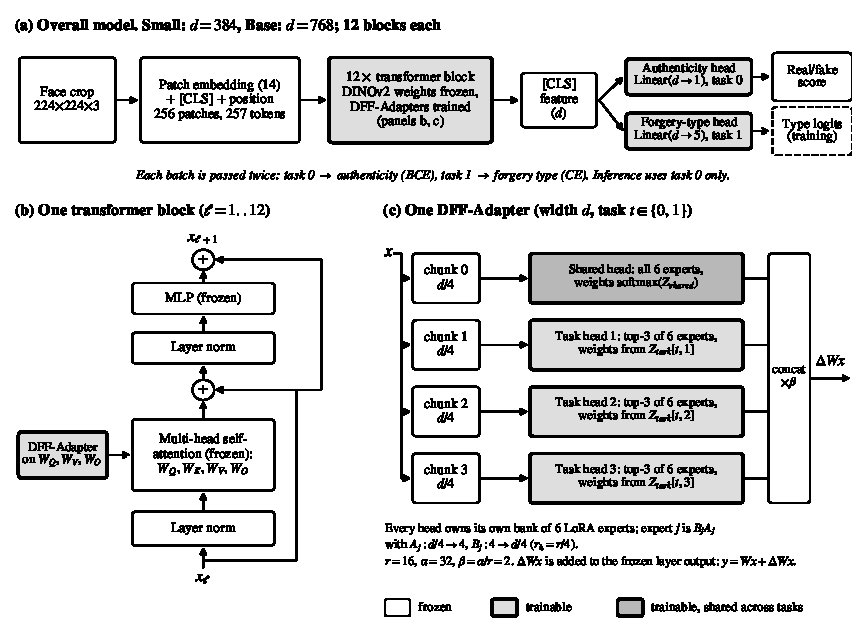
\includegraphics[height=0.66\textheight]{fig_arch}
\vspace{2pt}
\begin{itemize}\footnotesize
\item $\mathcal{L}=10\cdot\mathrm{BCE}(\text{auth})+2\cdot\mathrm{CE}(\text{type})$; two passes per batch; Small: 667{,}374 trainable parameters
\item Extension: type targets $(1-\epsilon)\,e_y+\epsilon/K$, $\epsilon=0.1$, type loss only
\end{itemize}
\end{frame}

\begin{frame}{Data and setup}
\small
\begin{tabular}{@{}p{0.47\textwidth}p{0.47\textwidth}@{}}
\textbf{Train / validate:} FF++ c23, 5{,}000 videos, 5 classes (original + 4 manipulations); MTCNN crops $224\times224$, 32 frames/video &
\textbf{Unseen test sets (all crops):}\\
\textbf{Config:} DINOv2-Small or Base (frozen), 12 or 30 epochs, 10 train / 8 val frames per video, batch 24, lr $10^{-4}$, weight decay 0.01, seed 42, Kaggle T4 &
Celeb-DF-v1: 100 videos, 3{,}200 frames\newline
Celeb-DF-v2: 518 videos, 16{,}576 frames\newline
DFDC subset: 392 videos (76 real / 316 fake), 12{,}544 frames\\
\end{tabular}
\vspace{4pt}
\begin{itemize}
\item Metrics: video AUC (primary, as in the paper), EER, frame AUC
\item Paper: DINOv2-Large, 50 epochs, lr $2\times10^{-4}$, weight decay $10^{-5}$, RTX 4090
\end{itemize}
\end{frame}

\begin{frame}{Main results: video-level AUC (\%)}
\centering
\footnotesize
\begin{tabular}{|l|c||c|c|c|c|}
\hline
Model & Ep. & FF++ & CDF-v1 & CDF-v2 & DFDC\\\hline
Small & 12 & 99.08 & 81.20 & 85.02 & --\\
\textbf{Small} & \textbf{30} & 99.08 & \textbf{82.98} & \textbf{86.25} & \textbf{88.03}\\
Small + LS 0.1 & 30 & 99.05 & 81.20 & 84.74 & 87.45\\
Base & 12 & 99.08 & 82.43 & 81.51 & --\\
Base & 30 & \textbf{99.16} & 81.71 & 84.22 & 84.00\\\hline
Paper (Base) & -- & 99.61 & n/r & 93.35 & 82.00\\
Paper (Large) & 50 & 99.56 & 96.14 & 95.26 & 89.96\\\hline
\end{tabular}
\vspace{6pt}
\begin{itemize}
\item Gap to paper (Large): 13.16 pp (CDF-v1), 9.01 pp (CDF-v2), but only 1.93 pp on our DFDC subset
\item FF++: our \emph{validation} AUC vs.\ paper's \emph{test} AUC (different splits)
\item ``--'': not evaluated, n/r: not reported by the paper
\end{itemize}
\end{frame}

\begin{frame}{Results at a glance}
\centering
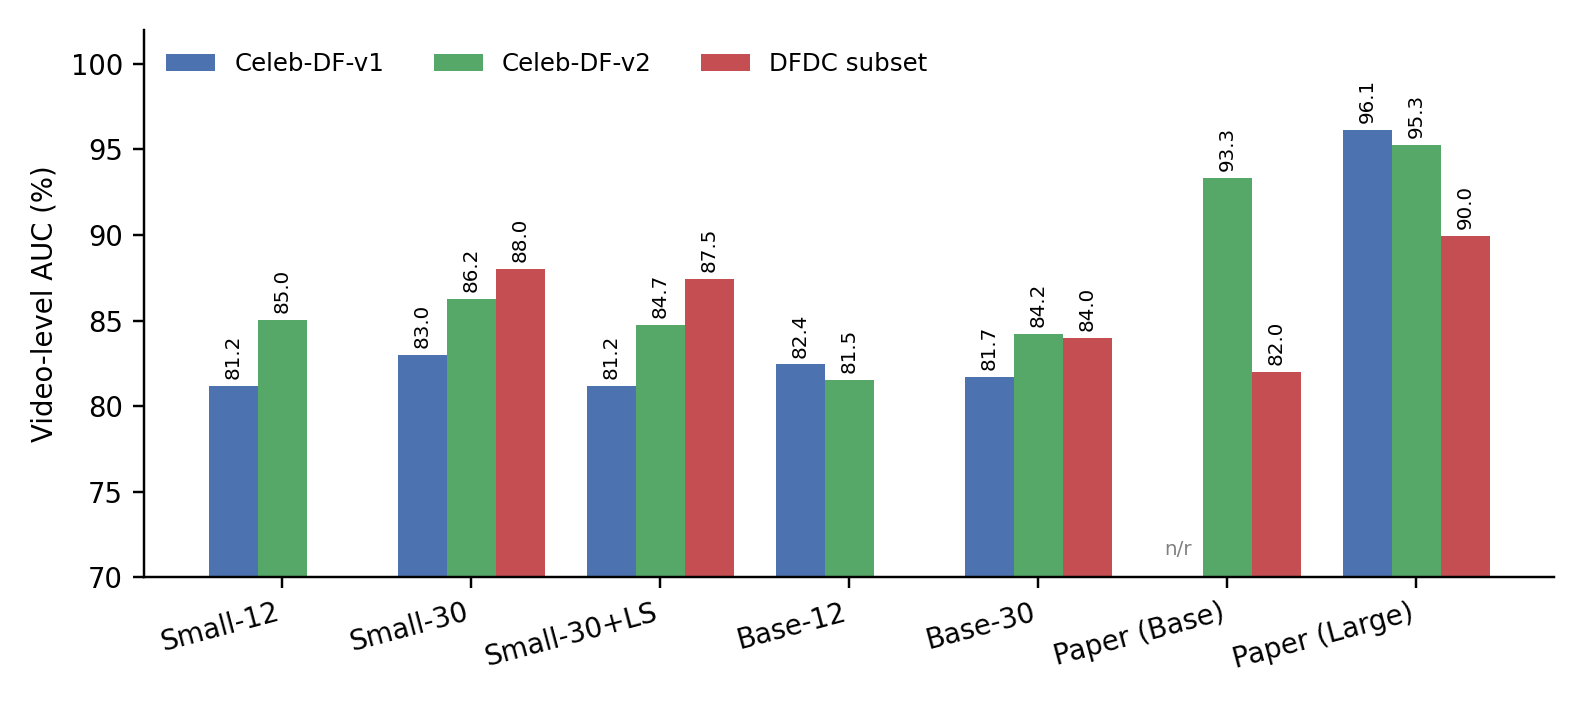
\includegraphics[height=0.72\textheight]{fig_auc}
\end{frame}

\begin{frame}{Equal Error Rate (\%) and DFDC detail}
\footnotesize
\begin{columns}[T]
\column{0.5\textwidth}
\centering
\begin{tabular}{|l|c||c|c|c|}
\hline
Model & Ep. & v1 & v2 & DFDC\\\hline
Small & 12 & 30.65 & 22.94 & --\\
\textbf{Small} & \textbf{30} & \textbf{26.32} & \textbf{22.35} & \textbf{19.74}\\
Small + LS & 30 & 26.32 & 25.00 & 19.94\\
Base & 12 & 25.81 & 26.18 & --\\
Base & 30 & 28.95 & 23.82 & 23.68\\\hline
Paper (Base) & -- & n/r & 14.61 & 25.49\\
Paper (Large) & 50 & n/r & 12.65 & 17.96\\\hline
\end{tabular}
\column{0.5\textwidth}
\centering
\begin{tabular}{|l||c|c|}
\hline
DFDC subset & Small & Base\\\hline
Video AUC & \textbf{88.03} & 84.00\\
EER & \textbf{19.74} & 23.68\\
Frame AUC & \textbf{79.99} & 78.10\\\hline
\end{tabular}
\end{columns}
\vspace{6pt}
\normalsize
\begin{itemize}
\item FF++ EER $\approx$3.2--3.6\% (val) vs.\ paper 1.79\% (test)
\item Video AUC $>$ frame AUC by 8.04 pp (Small), 5.90 pp (Base): aggregation damps noisy frames
\end{itemize}
\end{frame}

\begin{frame}{Ablation 1: training length and backbone size}
\footnotesize
\begin{columns}[T]
\column{0.52\textwidth}
\centering
\textbf{12 $\to$ 30 epochs} (change, pp)\\[3pt]
\begin{tabular}{|l||c|c|c|c|}
\hline
 & AUC v1 & EER v1 & AUC v2 & EER v2\\\hline
Small & $+1.78$ & $-4.33$ & $+1.23$ & $-0.59$\\
Base & $-0.72$ & $+3.14$ & $+2.71$ & $-2.36$\\\hline
\end{tabular}
\column{0.46\textwidth}
\centering
\textbf{Base minus Small, 30 ep.} (AUC, pp)\\[3pt]
\begin{tabular}{|l||c|}
\hline
Celeb-DF-v1 & $-1.27$\\
Celeb-DF-v2 & $-2.03$\\
DFDC & $-4.03$\\
FF++ val & $+0.08$\\\hline
\end{tabular}
\end{columns}
\vspace{6pt}
\normalsize
\begin{itemize}
\item Longer training helps Small; effect on Base depends on the target dataset
\item Larger backbone wins in-domain but not cross-dataset
\end{itemize}
\end{frame}

\begin{frame}{Ablation 2: label smoothing 0.1 on forgery-type loss}
\footnotesize
\centering
\begin{tabular}{|l||c|c|c|}
\hline
Small, 30 ep. (LS $-$ baseline) & $\Delta$ video AUC & $\Delta$ EER & $\Delta$ frame AUC\\\hline
Celeb-DF-v1 & $-1.78$ & $0.00$ & n/a\\
Celeb-DF-v2 & $-1.51$ & $+2.65$ & n/a\\
DFDC subset & $-0.58$ & $+0.20$ & $+0.91$\\\hline
\end{tabular}
\vspace{6pt}
\normalsize
\begin{itemize}
\item No gain in video AUC on any unseen set; DFDC frame AUC +0.91 pp
\item Single seed, and the baseline Celeb-DF numbers are final-checkpoint while LS used \texttt{best.pt}
\item Paper (Large): dropping the type loss costs 4.33 pp (CDF-v2) and 5.52 pp (DFDC); our no-aux, LoRA and linear-probe runs: \todo{results}
\end{itemize}
\end{frame}

\begin{frame}{Discussion}
\begin{columns}[T]
\column{0.5\textwidth}
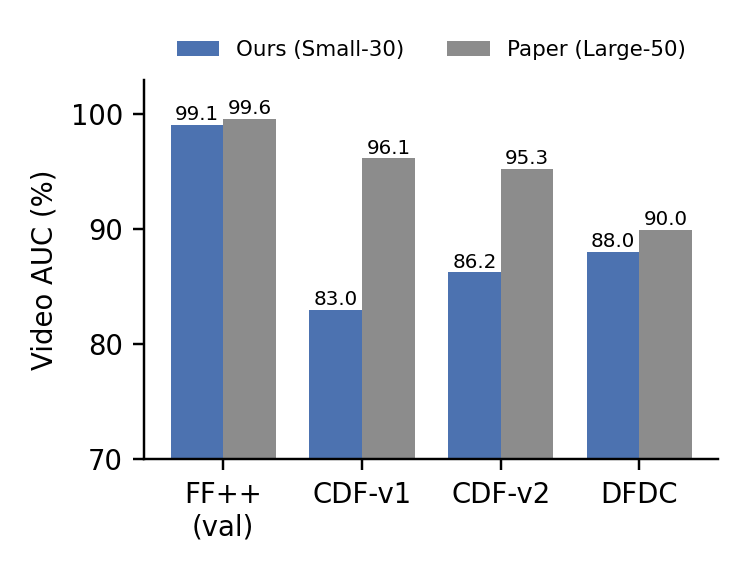
\includegraphics[width=\textwidth]{fig_gap}
\column{0.5\textwidth}
\begin{itemize}
\item In-domain accuracy $\ne$ robustness: $-16.10$ pp (v1), $-12.8$ pp (v2), $-11.05$ pp (DFDC) from FF++
\item Gap to paper is concentrated on Celeb-DF; causes (backbone, recipe, protocol, implementation) are not separable here
\item Bigger backbone and longer training do not guarantee better generalization
\end{itemize}
\end{columns}
\end{frame}

\begin{frame}{Limitations}
\small
\begin{itemize}
\item DINOv2-Small/Base instead of Large; different epochs, lr, weight decay, hardware
\item Splits not verified against the paper's; DFDC is a 392-video, imbalanced subset (76/316)
\item FF++ column is validation AUC (paper: test split)
\item Mixed checkpoints: FF++ best, baseline Celeb-DF final, DFDC and LS \texttt{best.pt}
\item Single seed; DFDC AUC 95\% interval $\approx\pm3.4$ pp (Hanley--McNeil), so 1--2 pp differences are within noise
\item Experiments show \emph{what} changes, not \emph{why}
\end{itemize}
\end{frame}

\begin{frame}{Conclusion and future work}
\textbf{Conclusions}
\begin{itemize}
\item FF++ AUC close (99.08\% val vs.\ 99.56\% test); Celeb-DF generalization not reproduced (82.98\% / 86.25\% vs.\ 96.14\% / 95.26\%); DFDC subset within 2 pp (88.03\% vs.\ 89.96\%)
\item Best of ours: Small, 30 epochs (88.03\% on the DFDC subset); Base and label smoothing did not help
\item Source-dataset performance alone is insufficient to judge a deepfake detector
\end{itemize}
\textbf{Next steps}
\begin{itemize}
\item One checkpoint evaluated on all four datasets; verify protocol; $\ge$3 seeds
\item One-factor ablations (adapter, type loss, smoothing); try Large and the paper's lr / weight decay
\end{itemize}
\end{frame}

\begin{frame}{References}
\footnotesize
\begin{thebibliography}{9}
\bibitem{a} T. Zhang et al., ``Fine-Grained DINO Tuning with Dual Supervision for Face Forgery Detection,'' AAAI, vol.~40, no.~15, pp.~12780--12788, 2026.
\bibitem{b} M. Oquab et al., ``DINOv2: Learning Robust Visual Features without Supervision,'' TMLR, 2024.
\bibitem{c} E. J. Hu et al., ``LoRA: Low-Rank Adaptation of Large Language Models,'' ICLR, 2022.
\bibitem{d} A. R\"ossler et al., ``FaceForensics++,'' ICCV, 2019.
\bibitem{e} Y. Li et al., ``Celeb-DF,'' CVPR, 2020.
\bibitem{f} B. Dolhansky et al., ``The DeepFake Detection Challenge (DFDC) Dataset,'' arXiv:2006.07397, 2020.
\end{thebibliography}
\end{frame}

\end{document}
